\documentclass[a4paper]{article}
\usepackage[a4paper, left=20mm, right=20mm, top=20mm, bottom=20mm]{geometry}
\usepackage[utf8]{inputenc}
\usepackage{indentfirst}
\usepackage{amsmath}
\usepackage{amssymb}
\usepackage{graphicx}
\usepackage{float}
\usepackage{amsthm}
\usepackage{authblk}
\usepackage{hyperref}

\DeclareMathOperator*{\argmin}{arg\,min}
\renewcommand{\footnoterule}{%
	\kern -3pt
	\hrule width \textwidth height 1pt
	\kern 2pt
}

\newcommand{\F}{\mathcal{F}}
\newcommand{\R}{\mathbb{R}}
\newcommand{\conv}{\rm{conv}\,}

\renewcommand{\baselinestretch}{1.3}

\theoremstyle{definition}
\newtheorem{definition}{Notation}[]

\title{CAQM: Convexity Analysis of Quadratic Maps}
\date{}
\author[1]{Anatoly Dymarsky\thanks{a.dymarsky@skoltech.ru}}
\author[1]{Elena Gryazina\thanks{e.gryazina@skoltech.ru}} 
\author[2]{Boris Polyak\thanks{boris@ipu.ru}}
\author[1]{Sergei Volodin\thanks{sergei.volodin@phystech.edu}}
\affil[1]{Skolkovo Institute of Science and Technology}
\affil[2]{Institute for Control Sciences RAS}

% fix ' character in verbatim
% see https://stackoverflow.com/questions/1662037/how-to-write-programming-code-containing-the-character-in-latex
\makeatletter
\let \@sverbatim \@verbatim
\def \@verbatim {\@sverbatim \verbatimplus}
{\catcode`'=13 \gdef \verbatimplus{\catcode`'=13 \chardef '=13 }}
\makeatother


\begin{document}
\newgeometry{left=30mm, right=30mm, top=30mm, bottom=30mm}
\maketitle
CAQM is a MATLAB library designed to analyze geometric properties of images of quadratic maps (which are manifolds of real-valued solutions of systems of quadratic equations).

This file is aimed at both guiding users with the installation steps and enumerating the methods and techniques which constitute the library. The main functionality described below is contained in several MATLAB functions located in the main folder.

Additional procedures which reside in the {\tt library/} folder are described in the accompanying file {\tt library.pdf}.

\newpage
\newgeometry{left=20mm, right=20mm, top=20mm, bottom=20mm}
\section*{Installation and Testing}
The library requires \href{https://www.mathworks.com/downloads/}{MATLAB} and \href{http://cvxr.com/cvx/download/}{CVX} as prerequisites. Having obtained those, the following steps are required in order to use CAQM.
\begin{enumerate}
\item {\bf Obtaining source code} can be done in two ways. First one requires basic knowledge of the GIT version control system. Simply clone the repository:
\begin{center}\tt
git clone git@github.com:sergeivolodin/CertificateCutting.git
\end{center}
The second option is to download the latest snapshot of the repository in form of a .zip archive. To do so, navigate to \href{https://github.com/sergeivolodin/CertificateCutting}{github.com/sergeivolodin/CertificateCutting}, press the green ,,Clone or download'' button and then choose ,,Download ZIP'' in the drop-down menu. Then unpack the obtained archive. Both cases should give a folder called {\tt CertificateCutting} (or {\tt CertificateCutting-master} in the latter case). This folder must contain a file {\tt README.md}.
\item {\bf Configuring MATLAB} involves adding the folder to the PATH. The following directories (assuming that the root folder is called {\tt CertificateCutting}) should be added: 

\begin{center}
{\tt CertificateCutting}, {\tt CertificateCutting/library}, {\tt CertificateCutting/tests}.
\end{center}

MATLAB gives two ways of adding a folder to MATLAB PATH. The first one involves \href{https://www.mathworks.com/help/matlab/ref/addpath.html}{console commands} and the second one \href{http://www.mathworks.com/help/matlab/ref/pathtool.html}{uses GUI}.
\item {\bf Testing the library} is an essential step which ensures that the library and all of its dependencies were installed correctly. To run the test, open MATLAB,

\begin{center}
navigate to {\tt CertificateCutting/tests} and run the {\tt testCAQM.m} file.
\end{center}

This file will go through essential parts of the functionality. During that period, a parallel cluster might be started (depending on the MATLAB version) and several GUI dialog boxes might be displayed. If the test succeeded, a message {\tt TEST PASSED} should be displayed in the console output. Otherwise, if the test has failed, a YouTube \href{https://youtu.be/Ikh_GDHnu-4}{video} demonstrating normal test operations might prove helpful in diagnosing the issue and overcoming installation mistakes. In other cases, feel free to contact the authors.

Moreover, there exist another group of tests which checks each function individually in a more thorough manner (run in MATLAB console from the {\tt CertificateCutting/tests} directory:
\begin{verbatim}
>> runtests('testFunctions')
\end{verbatim}
\end{enumerate}

After installation and testing, the library is ready to use in your applications. The sections below describe the functionality in details.

\newpage

\section*{Notations}
\begin{enumerate}
\item Real case, the map $f\colon \mathbb{R}^n\to\mathbb{R}^m$
\begin{equation}
f_k(x)=x^TA_k x+2b_k^Tx ,\quad A_k=A_k^T ,\quad x, b_k\in \mathbb{R}^n ,\quad i=k\dots m . \label{real}
\end{equation}
\item Complex case, the map $f\colon \mathbb{C}^n\to\mathbb{R}^m$
\begin{equation}
f_k(x)=x^*A_k x+b_i^*x+x^*b_k ,\quad A_k=A_k^* ,\quad x, b_k\in \mathbb{C}^n ,\quad i=k\dots m ,\label{complex}
\end{equation}
where $\cdot^*$ is Hermitian conjugate.
\end{enumerate}

We will use $\mathbb{V}$ to denote $\mathbb{R}^n$ in the real case and $\mathbb{C}^n$ in the  complex case.
We also use the following notations:\\

\theoremstyle{definition}
\begin{definition}
For a vector $c=(c_1,...,c_m)$ and a tuple of vectors $b=(b_1,...,b_m), \ b_k \in \mathbb{V}$, or a tuple of $n\times n$ matrices $A=(A_1,...,A_m), \  A_k\in \mathbb{V}^2$, the dot product is defined as follows,
\begin{eqnarray}
c\cdot b=\sum\limits_{k=1}^m c_k\, b_k ,\qquad
c\cdot A=\sum\limits_{k=1}^m c_k\, A_k\ . \nonumber
\end{eqnarray}
\end{definition}

\begin{definition}
The image of $f$ is denoted as $F$,
	$$F=f(\mathbb{V})\subset \mathbb{R}^m\ .$$
\end{definition}
\begin{definition} The convex hull of $F$ is denoted as $G$:
	$$G=\conv (F)\subset \mathbb{R}^m\ .$$
\end{definition}
\begin{definition} The boundary points of $F$ touched by a supporting hyperplane with the normal vector $c\in\mathbb{R}^m$,
	$$\partial F_c=\argmin\limits_{y\in F}(c\cdot y)$$
\end{definition}
\begin{definition} The boundary points of $G$ touched by a supporting hyperplane with the normal vector $c\in\mathbb{R}^m$,
	$$\partial G_c=\argmin\limits_{y\in G}(c\cdot y)$$
\end{definition}
\begin{definition}\label{ex:c_minus}
	Set of normal vectors $c$, such that $\partial F_c$ is non-convex is denoted as $C_-$,
	$$C_-=\{c\in\R^m\,\big|\,\mbox{Set }\partial F_c\mbox{ is non-convex}\}$$
\end{definition}

\newpage

\section*{Functionality}
The library consists of several functions, each of them is defined in a separate .m file.
Input format for specify the quadratic map is as follows.

\begin{itemize}
\item The array $A(i, j, k)$ denotes $i$'th row and $j$'th column of the $n\times n$ matrix $A_k\in\mathbb{V}^2$
\item The array $b(i, k)$ denotes $i$'th element of the vector $b_k\in\mathbb{V}$
\end{itemize}

\begin{enumerate}
\item {\bf Feasibility membership oracle,\hskip 6pt}\boxed{\tt \large  infeasibility\_oracle.m}
\begin{verbatim}
is_infeasible = infeasibility_oracle(A, b, y)
\end{verbatim}
{\bf Input:}
\begin{itemize}
\item The map $f$ specified by matrices $A_k$ and vectors $b_k$,
\item A point $y\in\mathbb{R}^m$.
\end{itemize}
{\bf Output:} determines if $y\in G$, returns {\tt is\_infeasible}=1 if $y\notin G$, {\tt is\_infeasible}=0 if $y\in G$.\\
{\bf Exceptions:} None

\begin{figure}[H]
	\centering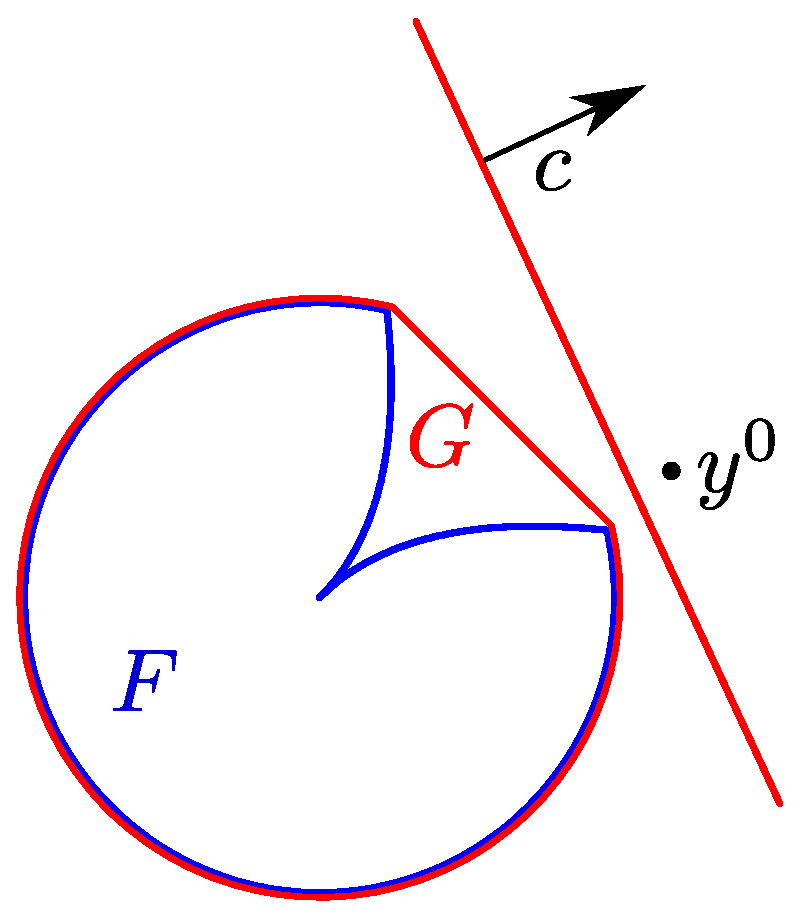
\includegraphics[width=100pt]{fig/infeasibility_oracle}
	\caption{Infeasibility oracle: hyperplane orthogonal to $c$ separates the point $y$ from the convex hull $G$ of $F$}
\label{fig:one}
\end{figure}

This function attempts to certify that the point $y$ does not belong to the convex hull $G$ of $F$ by separating $y$ and $G$ by an appropriate hyperplane.
This is illustrated in Fig.~\ref{fig:one}, see Theorem 3.2 in the accompanying article for details.

Procedure returns {\tt is\_infeasible}$=1$ if the desired hyperplane was found.
In this case $y\notin G$ and consequently $y\notin F$, implying there is no $x\in \mathbb{V}$ such that $y=f(x)$, i.e.~this point is infeasible.
If the hyperplane was not found the function returns {\tt is\_infeasible}$=0$, which means the feasibility  of $y$ with respect to $F$ is uncertain.
\newpage
\item {\bf Boundary oracle,\hskip 6pt}\boxed{\tt \large boundary\_oracle.m}
\begin{verbatim}
[t, is_in_F] = boundary_oracle(A, b, y, d)
\end{verbatim}
{\bf Input:}
\begin{itemize}
	\item The map $f$ specified by matrices $A_k$ and vectors $b_k$,
	\item A point $y\in G$,
	\item A direction $d\in\R^m$.
\end{itemize}
{\bf Output:}  finds and returns distance $t$ to the boundary of $G$ from the point $y$ inside $G$ in the direction $d$; verifies if the boundary point belongs to $F$.\\
{\bf Exception:}  if the input vector $y\notin G$ or in the case if $\partial G$ is not smooth at the boundary point $y+t\,d\in \partial G$, the function produces an exception.


\begin{figure}[H]
	\centering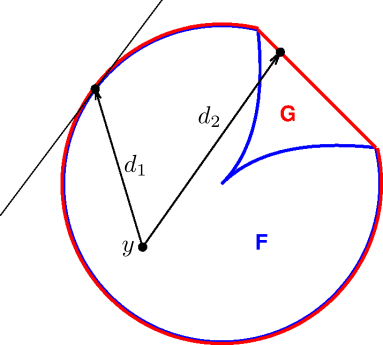
\includegraphics[width=100pt]{fig/boundary_oracle}
	\caption{Boundary oracle: distance from $y$ to the boundary $\partial G$ in the direction $d$.
	The boundary point of $G$ may or may not belong to $\partial F$ (cases of $d=d_1$ and $d=d_2$ respectively).}
\label{fig:two}
\end{figure}


This function finds point $y+t\,d$ on the boundary $\partial G$ with the largest $ {t} = \sup\{\tau\big| y+\tau d\in G\}$ and checks if this point belongs to $F$. 
This is illustrated in Fig.~\ref{fig:two}, see Optimization task (3) in the accompanying article for details.

The function returns $\tt t$ with the value of $t$, variable {\tt  is\_in\_F}$=1$ if the boundary point $y+t\,d$ belongs to $F$, and variable {\tt  is\_in\_F}$=0$ if feasibility of $y+t\,d$ with respect to $F$ is uncertain.

\newpage

\item {\bf Normal vector at the boundary,\hskip 6pt}\boxed{\tt get\_c\_from\_d.m} 
\begin{verbatim}
c = get_c_from_d(A, b, y, d)
\end{verbatim}
{\bf Input:}
\begin{itemize}
	\item The map $f$ specified by matrices $A_k$ and vectors $b_k$,
	\item A point $y\in G$,
	\item A direction $d\in\R^m$.
\end{itemize}
{\bf Output:}  finds point $y+t\,d$ at the boundary of $G$ and returns vector $c$ normal to $\partial G$ at that point\\
{\bf Exception:} if on the input $y\notin G$ or the normal vector to $\partial G$ at $y+td$ does not exist (because $\partial G$ is not smooth at this point)  the function produces an exception.


\begin{figure}[H]
	\centering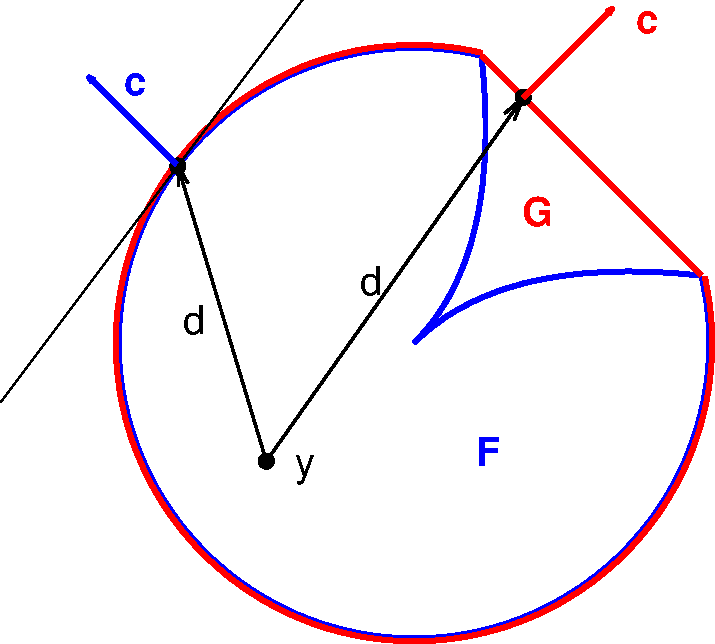
\includegraphics[width=100pt]{fig/get_c_from_d}
	\caption{Normal vector at the boundary: vector $c$ normal to $\partial G$ at the boundary point $y+td$. This function only considers the convex hull $G$ and does not distinguish between points $y+td$ which do or do not belong to $F$.}
\label{fig:three}
\end{figure}

This function finds the boundary point $y+td\in \partial G$ and calculates the vector $c$ normal to $\partial G$ at that point by using the dual formulation of the optimization problem, see equation (4) of the accompanying article.
This is schematically illustrated in Fig.~\ref{fig:three}.

The function returns vector variable $\tt c$ with the value of $c$.

\newpage

\item {\bf ``Non-convex direction",\hskip 6pt}\boxed{\tt \large get\_c\_minus.m} 
	\begin{verbatim}
	c = get_c_minus(A, b, [y], [k], [DEBUG])
	\end{verbatim}
{\bf Input:}
\begin{itemize}
	\item The map $f$ specified by matrices $A_k$ and vectors $b_k$,
	\item {\it (optional)} A point $y\in G$,
	\item {\it (optional)} Number of iterations $k$.
	\item {\it (optional)} Binary variable adding verbose output.
\end{itemize}
{\bf Output:}  finds and returns vector $c$ such that $\partial F_c$ is non-convex through a stochastic algorithm using up to $k$ iterations\\
{\bf Exception:} The functions throws an exception in the case if the vector $c$ was not found during the $k$ iterations

This function consequently generates up to $k$ random directions $d$ and for each one finds vector $c$ normal to $\partial G$ at the boundary point $y+t\, d\in \partial G$.
Next it finds $\partial F_c$, the intersection of $F$ with the supporting hyperplane orthogonal to $c$ and checks if it is non-convex.
We note that non-convexity of $\partial F_c$ implies non-convexity of $F$.
This function stops and returns $c$ if non-convexity of $\partial F_c$ was established during one of the iterations. If the vector $c$ was not found, an exception is produced.
If $y$ and $k$ are not specified, the function uses default values $y=f(0)=0$ and $k=10$.


\item {\bf Nonconvexity certificate,\hskip 6pt}\boxed{\tt \large nonconvexity\_certificate.m} 
	\begin{verbatim}
	is_nonconvex = nonconvexity_certificate(A, b, [y], [k])
	\end{verbatim}
{\bf Input:}
\begin{itemize}
	\item The map $f$ specified by matrices $A_k$ and vectors $b_k$,
	\item {\it (optional)} A point $y\in G$,
	\item {\it (optional)} Number of iterations $k$.
\end{itemize}
{\bf Output:} attempts to establish if $F$ is convex, returns {\tt is\_nonconvex}=$1$ if $F$ is non-convex,  {\tt is\_nonconvex}=$0$ if uncertain.
{\bf Exceptions:} None

	
This function calls {\tt get\_c\_minus} and returns  {\tt is\_nonconvex}=$1$ if the latter returns a non-trivial $c$. 


\item {\bf Positive-definite $c\cdot A$,\hskip 6pt}\boxed{\tt \large get\_c\_plus.m}
\begin{verbatim}
	c_plus = get_c_plus(A, [k], [DEBUG])
\end{verbatim}

{\bf Input:}
\begin{itemize}
	\item Matrices $A_k$
	\item {\it (optional)} The number of iterations $k$
	\item {\it (optional)} Binary variable adding verbose output.
\end{itemize}
{\bf Output:} finds and returns vector $c_+$ such that $c_+\cdot A\succ 0$.\\
{\bf Exception:} if $c_+$  was not found during $k$ iterations of the randomized procedure.
	
This function utilizes a randomized algorithm which is used to find $c_+$ such that $c_+\cdot A\succ 0$.

If successful, the function terminates and returns $c_+$ on the exit, otherwise the search attempt is repeated up to $k$ times.
If not specified explicitly, the default value of $k$ is $10$.
If $c_+$ is not found during $k$ iterations, the function produces an exception.

\newpage
	
\item {\bf Convex subpart,\hskip 6pt}\boxed{\tt \large get\_z\_max.m}
\begin{verbatim}
z_max = get_z_max(A, b, c_plus, [z_max_guess], [k], [DEBUG])
\end{verbatim}
{\bf Input:}
\begin{itemize}
	\item The map $f$ specified by matrices $A_k$ and vectors $b_k$,
	\item The vector $c_+$ such that $c_+\cdot A\succeq 0$,
	\item {\it (optional)} The guess value  $z^{\rm guess}_{\rm max}$,
	\item {\it (optional)} The number of iterations $k$.
	\item {\it (optional)} Binary variable adding verbose output.
\end{itemize}
{\bf Output:} finds and returns maximal value $z_{\max}$ such that the compact part of $F$ ``cut" by the hyperplane  $c_+ \cdot (y-y_0)=z_{\max}$, where $y_0\in \partial F_{c_+}$, is still convex. \\
{\bf Exception:} produces an exception if non-convexity of $F$ confined within the half-plane $c_+ \cdot (y-y_0)\leq z^{\rm guess}_{\rm max}$  has not been established, i.e. no non-convexities were found in that region.

\begin{figure}[H]
	\centering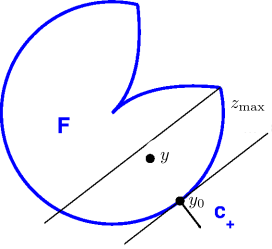
\includegraphics[width=100pt]{fig/get_z_max}
	\caption{Maximal value of $z_{\max}$ such that  the subpart of $F$, $F^{c_+}_{z_{\rm max}}\equiv \{y\, | y\in F, c_+ \cdot (y_0-y)\leq z_{\rm max}\}$, which is ``cut" from $F$ by a hyperplane orthogonal  to $c_+$ does not contain non-convexities.}
\label{fig:four}
\end{figure}


This function returns maximal value $z_{\max}$ such that the hyperplane perpendicular to $c_+$ and located distance $z_{\max}$ away from the boundary of $F$ still does not contain non-convexities.
More precisely, the compact part of $F$ confined by the half-space $\{y\, |c_+ \cdot (y_0-y)\leq z^{\rm guess}_{\rm max}\}$ is convex.
Here $y_0\in \partial F_{c_+}$, and since $c_+\cdot A\succ 0$, the set $\partial F_{c_+}$ is a singleton $\{y_0\}$.
Moreover, $z_{\max}$ is maximal in a sense that enlarging it would result in the resulting ,,cut'' containing at least one boundary non-convexity, which are non-convex subsets of the boundary $\partial F_c$ defined as the points touched by a hyperplane with a normal vector $c$.
The geometric meaning of $z_{\max}$ is illustrated in Fig. \ref{fig:four}. 

The function first tries to identify ``non-convex directions" $c_-$ using {\tt get\_c\_minus} and then ``follow" each non-convexity to the smallest value of $z$. This is described in detail in the section 4.4 of the accompanying paper.

If no ``non-convex directions" found, the function produces an exception.
In case the input value of $c_+$ does not satisfy $c_+\cdot A\succ 0$, the function produced as exception.
If the maximal number of iterations $k$ (to be used with {\tt get\_c\_minus}) is not specified on input, a heuristic default value $k=10$ is used.

The guess value $z^{\rm guess}_{\rm max}$ is supposed to be substantially large to detect non-convexity of $F$.
If it is not specified on input, a default value of $z^{\rm guess}_{\rm max}=10 {\rm Tr}(c_+\cdot A)$ is used.

It is important to keep in mind that the algorithm is heuristic.
A non-trivial return value $z_{\max}\neq z^{\rm guess}_{\rm max}$ does not guarantee convexity of  $F_{z_{\rm max}}\equiv \{y\, | y\in F, c_+ \cdot (y_0-y)\leq z_{\rm max}\}$, but only that $\{y\, | y\in F,c_+ \cdot (y_0-y)\leq z\}$ for any $z>z_{\rm max}$ contains boundary non-convexities.
Nevertheless, increasing $k$ would increase certainty (in the probabilistic sense) that $F_{z_{\rm max}}$ is indeed convex. 

\end{enumerate}
\end{document}
